\documentclass{article}
\usepackage[utf8]{inputenc}
\usepackage[T1]{fontenc}
\usepackage{amsmath,amssymb}
\usepackage{pgfplots}
\usepackage{tikz}
\usepackage{lmodern}
\usepackage{graphicx}
\usepackage{hyperref}
\usepackage{listings}
\usepackage{xcolor}
\usepackage{enumitem}
\usepackage{fancyhdr}
\usepackage{lastpage}
\usepackage[left=2.5cm,right=2.5cm,top=2.5cm,bottom=2.5cm]{geometry}
\usepackage[table]{xcolor}
\usepackage{array}
\usepackage{hyperref}
\usepackage{nameref}

\pagestyle{fancy}
\fancyhf{}
\renewcommand{\headrulewidth}{0pt}
\rfoot{\thepage\ af \pageref{LastPage}}

\title{Forløbsplan}
\author{Anders S. Østergaard}
\date{\today}

\definecolor{codegreen}{rgb}{0,0.6,0}
\definecolor{codegray}{rgb}{0.5,0.5,0.5}
\definecolor{codepurple}{rgb}{0.58,0,0.82}
\definecolor{backcolour}{rgb}{0.95,0.95,0.92}
\definecolor{darkerlightblue}{rgb}{0.1, 0.3, 0.5}

\lstdefinestyle{mystyle}{
	backgroundcolor=\color{backcolour},   
	commentstyle=\color{codegreen},
	keywordstyle=\color{darkerlightblue},
	numberstyle=\tiny\color{codegray},
	stringstyle=\color{codepurple},
	basicstyle=\ttfamily\footnotesize,
	breakatwhitespace=false,         
	breaklines=true,                 
	captionpos=b,                    
	keepspaces=true,                 
	numbers=left,                    
	numbersep=5pt,                  
	showspaces=false,                
	showstringspaces=false,
	showtabs=false,                  
	tabsize=2
}
\lstset{style=mystyle}
\usepackage{float}
\usepackage{xcolor}
\usepackage{pdfpages}
\usepackage{subcaption}
\begin{document}
	\begin{titlepage}
	\centering
	\vspace*{6cm}
	{\Huge\bfseries SWROB2\par Exam\par}
	\vspace{2cm}
	Submitted by: \par 
	\begin{table}[!h]
		\centering
		\begin{tabular}{|l|l|l|}
			\hline
			Study nr  & Name 					   & Study line\\\hline
			202005180 & Nicolaj Meldgaard Pedersen & E\\\hline
			202105443 & Johannes Baagøe 		   & E\\\hline
			201270449 & Anders Sandø Østergaard    & EP\\\hline
			201905293 & Daniel F. Borch Olsen	   & E\\\hline
		\end{tabular}
	\end{table}
	\vspace{4cm}
	Århus Universitet \par
	\vfill
	\today
\end{titlepage}
\pagenumbering{arabic}
\thispagestyle{empty}
\begin{abstract}
	\textit{This report presents the design, implementation, and evaluation of an advanced robotic system integrated with the Robot Operating System (ROS). The project leverages ROS's dynamic capabilities alongside sophisticated algorithms to enhance robotic functionalities in motion control, motion planning, perception using camera algorithms, localization, and mapping. Utilizing MATLAB and a specific hardware setup, the system demonstrates significant improvements in task efficiency and obstacle management within a controlled experimental setup. The findings highlight the system’s robustness in real-time operations and its potential for adaptation in varied automation scenarios. This study not only showcases the successful application of ROS in complex robotic tasks but also sets a foundation for future advancements in robotic automation. The report concludes with an analysis of experimental results, discussing the system's performance against predefined objectives and suggesting areas for further research.}
\end{abstract}
\clearpage
\tableofcontents
\clearpage
	\clearpage
	
	\section{Introduction}
	In recent years, the integration of robotics into industrial and research applications has significantly advanced, driven by innovations in robotics operating systems and algorithm development. One of the most utilized platforms is the Robot Operating System (ROS), which provides tools and libraries designed to support the development of robot behavior. This report focuses on a robotics system designed to sense, plan, and act within Shannon, a building at Aarhus University. By using Matlab and ROS then we will demonstrate how motion control, planning, perception, localization, and mapping will be the core of an autonomous mobile robot.
	\\\\
	The primary objective of this project is to develop and evaluate a robot system that effectively demonstrates the capabilities of various algorithms in a controlled environment. By utilizing ROS and other software tools, such as Matlab, coupled with a selected hardware setup, the project aims to control and navigate a TurtleBot3 from a start location to an ending location while doing tasks along the way.
	\\\\
	\noindent This report will cover several key aspects:
	\begin{enumerate}
		\item \textbf{Robot System Description:} An in-depth look at the overall setup, including detailed descriptions of the hardware and software components utilized in the project.
		\item \textbf{Principles of ROS:} An explanation of how ROS operates, focusing on its architecture and the communication patterns that facilitate multi-component integration in robotics projects.
		\item \textbf{Algorithms:} A discussion on the core algorithms developed and implemented, detailing their design, objectives, and impact on the system’s performance.
		\item \textbf{Discussion and Conclusion:} Insights derived from the project outcomes, including an assessment of the system's performance and recommendations for future enhancements.
	\end{enumerate}
	The subsequent sections will delve into each of these areas, providing an overview of the project. 
	
	\section{Task}
	The description of task provided by the school will not be presented here but you would be advised to be reading it in the appendix \ref*{appendix:task}.
	
	\subsection{Resume of the task Sequence}
	The tasks to be performed by the TurtleBot are as follows:
	\begin{enumerate}
		\item The robot must always start at location \textcolor{red}{A}.
		\item The robot must drive autonomously from location \textcolor{red}{A} to location \textcolor{green}{B}, avoiding any obstacles along its path.
		\item Upon reaching location \textcolor{green}{B}, the robot must automatically locate a red circle on a white piece of paper, on a wall.
		\item After identifying the red circle, the robot must position itself 50 cm in front of the marker and take a photograph and store it.
		\item Subsequently, the robot must navigate autonomously to location \textcolor{blue}{C} using a path-planning algorithm to find the best route.
		\item At location \textcolor{blue}{C}, the robot must locate a purple circle on a white piece of paper on a wall.
		\item Upon locating the purple circle, the robot should position itself 50 cm in front of the marker and take a photograph and store it.
	\end{enumerate}

	\section{Robot System Description}
	\subsection{Description of the Setup}
	This project utilizes the TurtleBot3, a popular and versatile platform widely used in robotics education and research. The TurtleBot3 is known for its modular design and compatibility with various ROS versions, making it an ideal candidate for demonstrating robotics algorithms for educational use. The robot is tasked with performing a series of autonomous operations, including navigation, obstacle avoidance, and object recognition, within a controlled environment designed to simulate real-world conditions. The setup includes a predefined track with various obstacles and visual markers to challenge the robot's perception and motion planning capabilities.
	
	\subsection{Hardware/Software Used}
	The hardware foundation of the TurtleBot3, equipped with standard sensors such as Lidar for mapping and navigation, camera module for visual perception tasks. The primary software components include:
	\begin{itemize}
		\item \textbf{ROS1 Noetic:} The latest long-term support version of ROS1, serving as the middleware that facilitates communication between the robot's hardware components and high-level algorithms.
		\item \textbf{MATLAB:} Used for developing some of the robot's algorithms, especially in areas related to image processing and data analysis. MATLAB's integration with ROS allows for direct communication between the MATLAB scripts and ROS topics, enhancing the system's ability to perform complex calculations and algorithm testing efficiently.
	\end{itemize}
	
	\subsubsection*{Hardware}
	\begin{itemize}
		\item \textbf{TurtleBot3 Robot:} The core of the project, the TurtleBot3, is a compact and customizable mobile robot platform compatible with various ROS versions. It is specifically designed for education and research in robotics. The model used in this project is the TurtleBot3 Burger, which includes the following components:
		\begin{itemize}
			\item \textbf{Raspberry Pi 3:} Serves as the main control unit.
			\item \textbf{360-degree LiDAR sensor:} For environmental scanning and obstacle avoidance.
			\item \textbf{Camera (USB):} Used for visual object and obstacle detection.
			\item \textbf{Dynamixel motors:} Provide precise and powerful actuation for movement.
			\item \textbf{Inertial measurement units (IMUs):} Provides orientation and motion detection.
	\end{itemize}
	\end{itemize}
	
	\subsubsection*{Software}
	\begin{itemize}
		\item \textbf{ROS Noetic:} The Robot Operating System (ROS) serves as the middleware that offers a suite of tools and libraries designed to facilitate the development of robot applications. ROS Noetic, specifically tailored for long-term support versions of Ubuntu, such as 20.04 LTS.
		\item \textbf{MATLAB:} Utilized for advanced algorithm development, data analysis, and visualization, MATLAB integrates seamlessly with ROS, allowing for easy implementation of advanced control strategies. The Robotics System Toolbox in MATLAB is particularly used to prototype, test, and run these algorithms efficiently.
	\end{itemize}
	
	\section{Principles of ROS}
	\subsection{Robot Operating System (ROS)}
	The Robot Operating System (ROS) is an open-source framework for writing robot software. It provides a structured communications layer above the host operating systems of a mixed compute cluster. ROS's utilities, libraries, drivers, conventions, and tools are designed to simplify the task of creating complex and robust robot behavior across a wide variety of robotic platforms. ROS is not an operating system in the traditional sense of process management and scheduling; instead, it provides a structured framework that supports the development of distributed computing solutions.
	
	\subsection{Topics}
	Topics are named buses over which nodes exchange messages. Communication on topics happens via a publish/subscribe mechanism where nodes send messages (publish) without knowing who, if anyone, will receive them, and receive messages (subscribe) without knowing who, if anyone, has sent them. This model is particularly well-suited for streaming data, such as sensor readings and control signals where it is not critical to handle every message that comes through.
	
	\subsection{Messages}
	Messages are simple data structures, comprising typed fields. They can include arrays and constants and are used to send data among nodes. Each topic and service uses a specific message type, which is a data structure predetermined by the sender and receiver in the communication process. ROS supports complex message structures, allowing a wide variety of information to be passed between nodes.
	
	\subsection{Publisher}
	A publisher is, a function, inside a node that creates messages to a specific topic in a ROS network. Publishers declare the topic on which they will publish, the type of message they will send, and then publish messages to anyone who is subscribed to this topic. This setup allows for real-time data sharing.
	
	\subsection{Subscriber}
	A subscriber is, a function inside a node that receives messages from a specific topic in a ROS network. Subscribers declare the topic they want to receive and the type of message it is. They are then responsible for handling these messages as they arrive. This mechanism is vital for nodes that need to perform actions based on data from other parts of the system, such as processing sensor inputs or executing commands based on received instructions.
	
	\subsection*{Graphical overview for TurtleBot3}
	The following figure is showing some of the topics inside TurtleBot3.
	\begin{figure}[h]
		\centering
		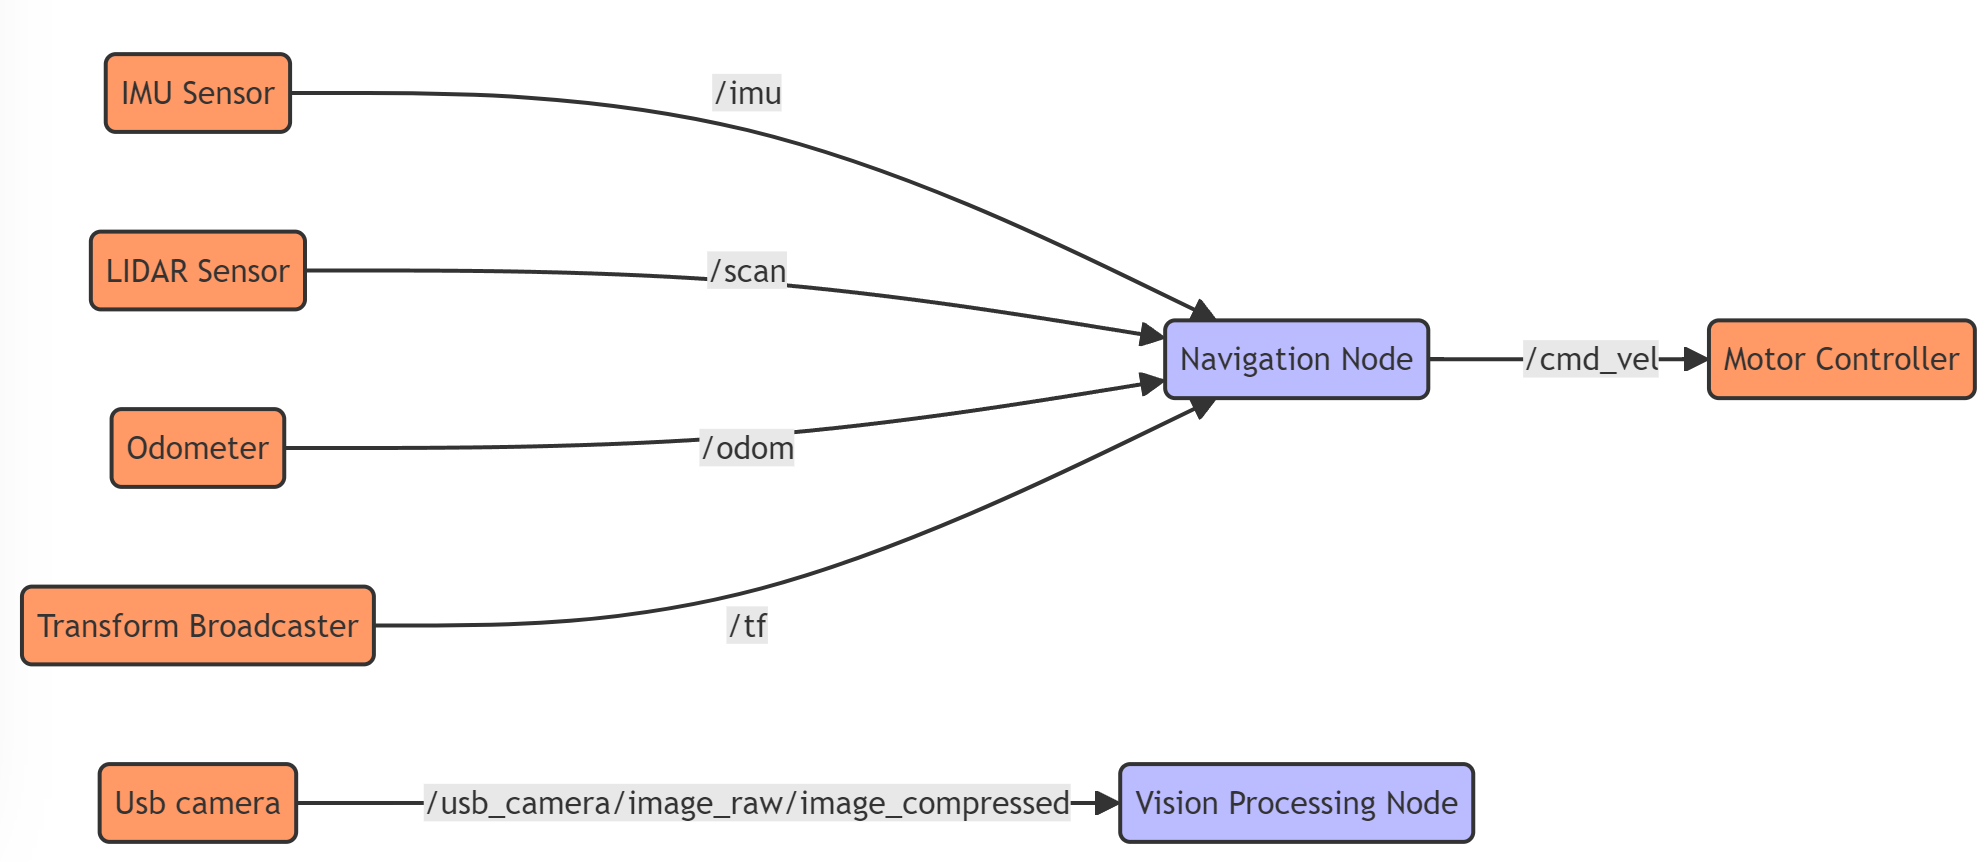
\includegraphics[width=0.6\linewidth]{fig/fig4.png}
		\caption{This diagram provides an accurate description of the used topics that we did find relevant for this project.}
	\end{figure}
	\clearpage
	\begin{itemize}
		\item \textbf{IMU Sensor (\texttt{/imu})}: Used to measure linear and rotational acceleration, crucial for robot stability and orientation.
		
		\item \textbf{USB Camera RGB (\texttt{/usb\_cam/image\_raw/compressed})}: Provides visual data from the usb camera that was attached to the robot for the node passing it to Matlab.
		
		\item \textbf{LIDAR Sensor (\texttt{/scan})}: Essential for measuring distances and detecting obstacles, aiding the navigation system in avoiding obstacles and planning safe routes.
		
		\item \textbf{Odometer (\texttt{/odom})}: Provides data about the robot's movement and position based on the serve motor encoders, essential for accurate localization and navigation.
		
		\item \textbf{Transform Broadcaster (\texttt{/tf})}: Manages coordinate transformations between different reference frames on the robot, necessary for accurate positioning and movement.
		
		\item \textbf{Motor Controller}: Receives and executes commands to the robot's motors, based on input from the navigation system.
	\end{itemize}
	\section{Algorithms}
	\subsection{Motion control}
	\subsubsection{Pure Pursuit Algorithm}
	The Pure Pursuit algorithm is a geometric path tracking method commonly used in autonomous robotics and self-driving vehicles to follow a predefined path. The algorithm calculates the required steering angle to follow a path by continuously chasing a point ahead on the path, which is why it's called "pure pursuit."
	
	\subsubsection*{Basic Concept}
	The fundamental idea behind the Pure Pursuit algorithm is relatively simple:
	\begin{enumerate}
		\item A look-ahead point is dynamically chosen on the path at a fixed distance ahead of the current position of the robot or vehicle.
	
		\item The algorithm then calculates the curvature (steering angle) required for the vehicle to travel in a circular arc to reach this look-ahead point.
		
		\item The curvature is recalculated at each update step as the vehicle progresses along the path, ensuring dynamic adjustment to the path's shape and the vehicle's current state.
	\end{enumerate}
		\begin{figure}[!h]
		\centering
		\begin{subfigure}[b]{0.3\textwidth}
			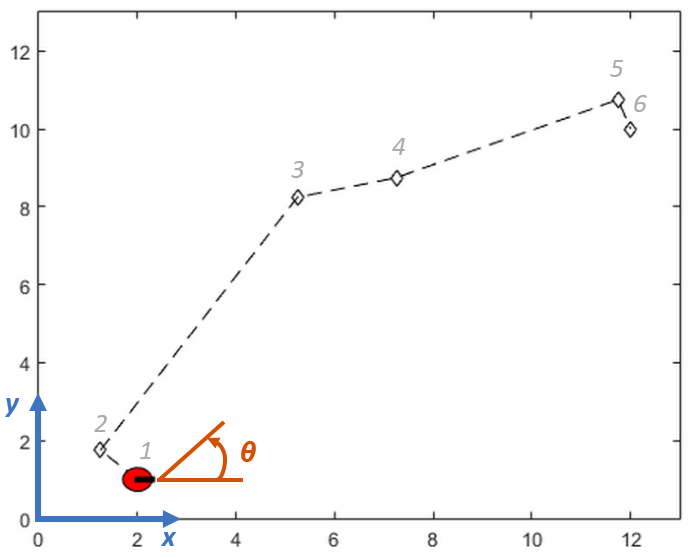
\includegraphics[width=\textwidth]{fig/fig5.png}
			\caption{Reference Coordinate System}
			\label{fig:image1}
		\end{subfigure}
		\hfill
		\begin{subfigure}[b]{0.3\textwidth}
			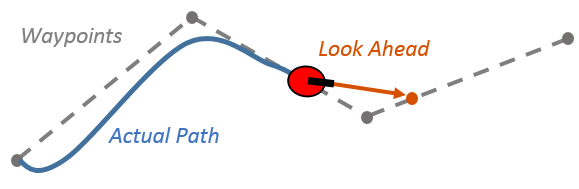
\includegraphics[width=\textwidth]{fig/fig6.png}
			\caption{Look Ahead Distance}
			\label{fig:image2}
		\end{subfigure}
		\hfill
		\begin{subfigure}[b]{0.3\textwidth}
			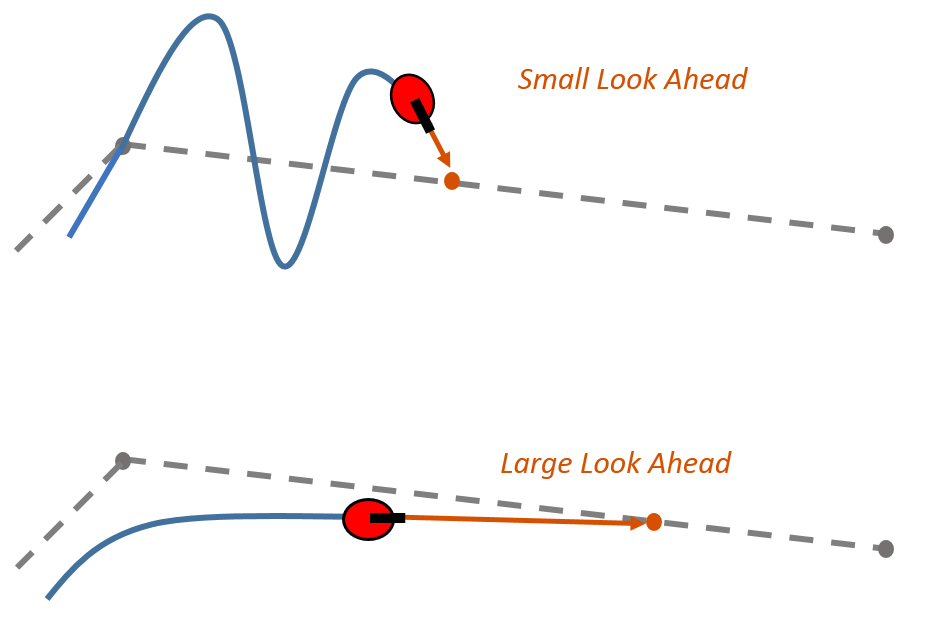
\includegraphics[width=\textwidth]{fig/fig7.png}
			\caption{Small and large look ahead distance}
			\label{fig:image3}
		\end{subfigure}
		\caption{Showing the reference coordinate system along with effect of having too short or large distance between waypoints}
		\label{fig:three_images}
	\end{figure}
	\subsubsection*{Implementation}
	The following code snippet demonstrates the implementation of the Pure Pursuit algorithm in MATLAB for a robot:
	\begin{verbatim}
		% Controller setup
		controller = controllerPurePursuit;
		controller.DesiredLinearVelocity = 0.2;
		controller.MaxAngularVelocity = 2;
		
		% We found that the robot is relatively stable with a LookAheadDistance of 0.4
		controller.LookaheadDistance = 0.4;
		
		% Since we're using the reference frame of the LIDAR, position and angle are always 0
		first_PRM = createFirstPRM();
		second_PRM = createSecondPRM();
	\end{verbatim}
	
	\subsubsection*{Explanation}
	\begin{itemize}
		\item \textbf{Controller Setup:}
		\begin{itemize}
			\item The \texttt{controllerPurePursuit} object is created to manage the Pure Pursuit controller.
			\item \texttt{DesiredLinearVelocity} is set to \texttt{0.2} which defines the speed at which the robot will move.
			\item \texttt{MaxAngularVelocity} is set to \texttt{2} which limits the maximum rate of change of the steering angle.
		\end{itemize}
		\item \textbf{Lookahead Distance:}
		\begin{itemize}
			\item The \texttt{LookaheadDistance} is set to \texttt{0.4}. This distance is crucial for the stability of the robot's path-following behavior. It determines how far ahead the robot looks on the path to choose the next point to move towards.
		\end{itemize}
		\item \textbf{Reference Frame:}
		\begin{itemize}
			\item Since the reference frame is based on the LIDAR's position, the position and angle are always set to \texttt{0}. This simplifies the calculations as it aligns the robot's reference frame with the path's reference frame.
		\end{itemize}
		\item \textbf{PRM Paths:}
		\begin{itemize}
			\item \texttt{first\_PRM} and \texttt{second\_PRM} are paths generated by the Probabilistic Roadmap (PRM) algorithm. These paths are used by the Pure Pursuit controller to navigate the environment.
		\end{itemize}
	\end{itemize}
	This implementation ensures that the robot dynamically adjusts its path by recalculating the curvature at each update step, allowing it to follow the defined path smoothly.
	\\\\
	\noindent The PRM Paths will be covered in another section.
	
	
	\subsubsection*{Advantages and Limitations}
	\textbf{Advantages:}
	\begin{itemize}
		\item \textbf{Simplicity:} The Pure Pursuit algorithm is straightforward to implement and understand.
		\item \textbf{Effectiveness:} It is very effective for smooth paths and can be implemented in real-time applications due to its computational efficiency.
	\end{itemize}
	\textbf{Limitations:}
	\begin{itemize}
		\item \textbf{Performance in Sharp Turns:} The algorithm may struggle with very sharp turns or abrupt path changes because it only considers the current look-ahead point without anticipating future path changes.
%		\item \textbf{Dependency on Look-ahead Distance:} The choice of look-ahead distance can greatly affect the performance of the algorithm, requiring careful tuning based on specific vehicle dynamics and path characteristics.
	\end{itemize}
	
%	\subsubsection*{Applications}
%	The Pure Pursuit algorithm is extensively used in scenarios where path tracking is crucial, such as in autonomous vehicles, unmanned ground vehicles in agriculture, or robotic systems in industrial settings.
%	\\\\
%	In conclusion, while the Pure Pursuit algorithm has some limitations, its simplicity and effectiveness make it a popular choice for real-world applications requiring robust path following capabilities under varying operational conditions.
	
	\section{Camera-Based Perception for Circle Detection}
	Camera-based perception algorithms are crucial for enabling autonomous robots to detect and interact with objects in their surroundings. In this section, we will focus on the specific task of detecting colored circles in images captured by the robot's camera.
	
	\subsection{Overview of Circle Detection}
	In robotic systems, cameras provide high-dimensional data that can be processed to extract meaningful information. The processing of this data is achieved through various image processing techniques:
	\begin{itemize}
		\item \textbf{Image Processing:} Basic manipulation of images to enhance the visibility of features, such as edge detection and filtering.
		\item \textbf{Color Segmentation:} Identifying specific colors within the image to isolate regions of interest.
		\item \textbf{Shape Detection:} Detecting geometric shapes, such as circles, using algorithms designed for shape recognition.
	\end{itemize}
	
	\subsection{Implementation of Circle Detection Algorithm}
	To be making a complete overview of the code used for detecting both red and purple circles will take too much space and therefore we advice you to be reading the Appendix~\ref{appendix:code} for a more detailed explanation. In this section we will cover the steps we go through for detecting both colors by using a flowchart.
	\begin{itemize}
		\item Step 1: receiving from subscription of the topic "/usb\_cam/image\_raw/compressed"
		
		\item Step 2: Rotating the image 180 degree and bilinear interpolation.
		
		\item Step 3: Storing the image.
		
		\item Step 4: Converting the image from RGB to HVS for making it easier to detecting red and purple.
		
		\item Step 5: Defining thresholds for hue, saturation, and value channel.
		
		\item Step 6: Create a kernel using the threshold values.
		
		\item Step 7: Combining the three kernels to one kernel.
		
		\item Step 8: Applying the kernels on the original image.
		
		\item Step 9: Making erosion for closing all holes.
		
		\item Step 10: Making dilation. Opening all holes. By making a erosion before dilation is filtering noise from the image.
		
		\item Step 11: Converting to gray scale
		
		\item Step 12: Converting to binary by using threshold. By having a binary image it's easier be detecting circles.
		
		\item Step 13: Detecting circle. If circle proceed to "step 14: Confidence Check" else proceed to "Step 15: No circle Found"
		
		\item Step 14: Confidence Check. If the value "Confidence > 0.3" proceed to "Step 16: Display Image" else proceed "Step 15: No circle Found"
		
		\item Step 15: No circle Found.
		
		\item Step 16: Display Image
		
		\item Step 17: End.
	\end{itemize}
	\begin{figure}[!h]
		\centering
		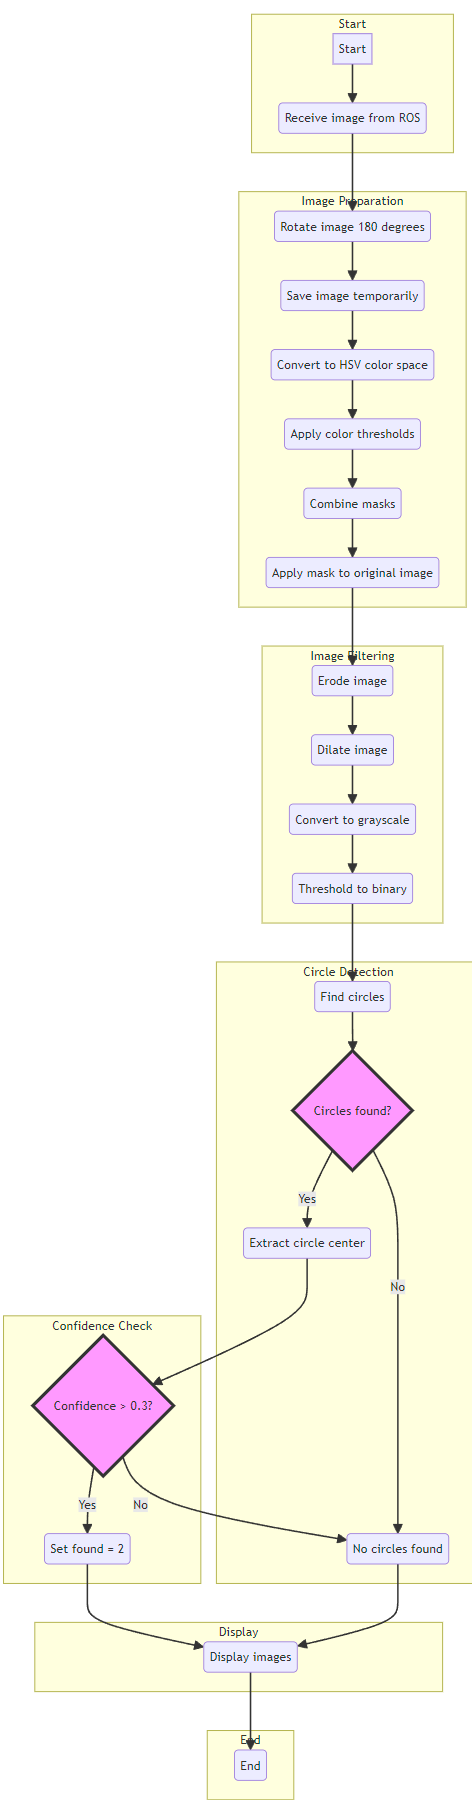
\includegraphics[width=.25\textheight]{fig/fig9.png}
		\caption{Flowchart for the color detection}
	\end{figure}
	\clearpage
	\section{Localization}
	Localization is a fundamental aspect of autonomous robotics, enabling a robot to determine its position within an environment. In the context of the final project, the TurtleBot must accurately identify its location within the Shannon building to navigate between specified points and perform tasks effectively.
	
	\subsection{Project Requirements and Localization Strategy}
	The project requires the TurtleBot to start at a fixed location (Location A) and autonomously travel to Locations B and C to perform specific tasks. The sequence of tasks includes object recognition and navigation around obstacles, demanding precise and reliable localization capabilities. The key steps involving localization are:
	
	\begin{enumerate}
		\item \textbf{Initial Positioning:} The robot starts from Location A. Initial localization is straightforward, as the starting point is predefined and known.
		\item \textbf{Navigation to Location B:} The robot must autonomously navigate from Location A to B, avoiding any obstacles. This requires dynamic localization to continually update the robot's current position and adjust its path.
		\item \textbf{Object Recognition and Position Adjustment at Location B:} Upon arriving at B, the robot must locate a red circle on the wall, approach it to a distance of 50 cm, and take a picture. This task requires the robot to fine-tune its localization to position itself precisely relative to the target object.
		\item \textbf{Path Planning to Location C:} After completing the task at Location B, the robot must find the optimal route to Location C. This involves complex path planning algorithms that depend on accurate localization to navigate around static and dynamic obstacles.
		\item \textbf{Object Recognition and Position Adjustment at Location C:} Similar to Location B, the robot must locate a purple circle, approach, and photograph it. This again requires precise localization to successfully complete the task.
	\end{enumerate}
	
	\subsection{Techniques and Tools for Effective Localization}
	To achieve effective localization, several techniques and tools are employed:
	\begin{itemize}
		\item \textbf{Odometry:} Utilized to estimate the robot's change in position over time. This is achieved by interpreting data from wheel encoders.
		\item \textbf{Probabilistic Roadmap (PRM):} Used for path planning, PRM helps in determining a feasible path from one location to another by randomly sampling the environment and creating a roadmap of possible paths.
		\item \textbf{Sensors:} The TurtleBot uses a combination of sensors, including LiDAR for obstacle detection and a camera for visual identification of the target markers (red and purple circles).
	\end{itemize}
	\begin{figure}[!h]
		\centering
		\begin{subfigure}[b]{0.45\textwidth}
			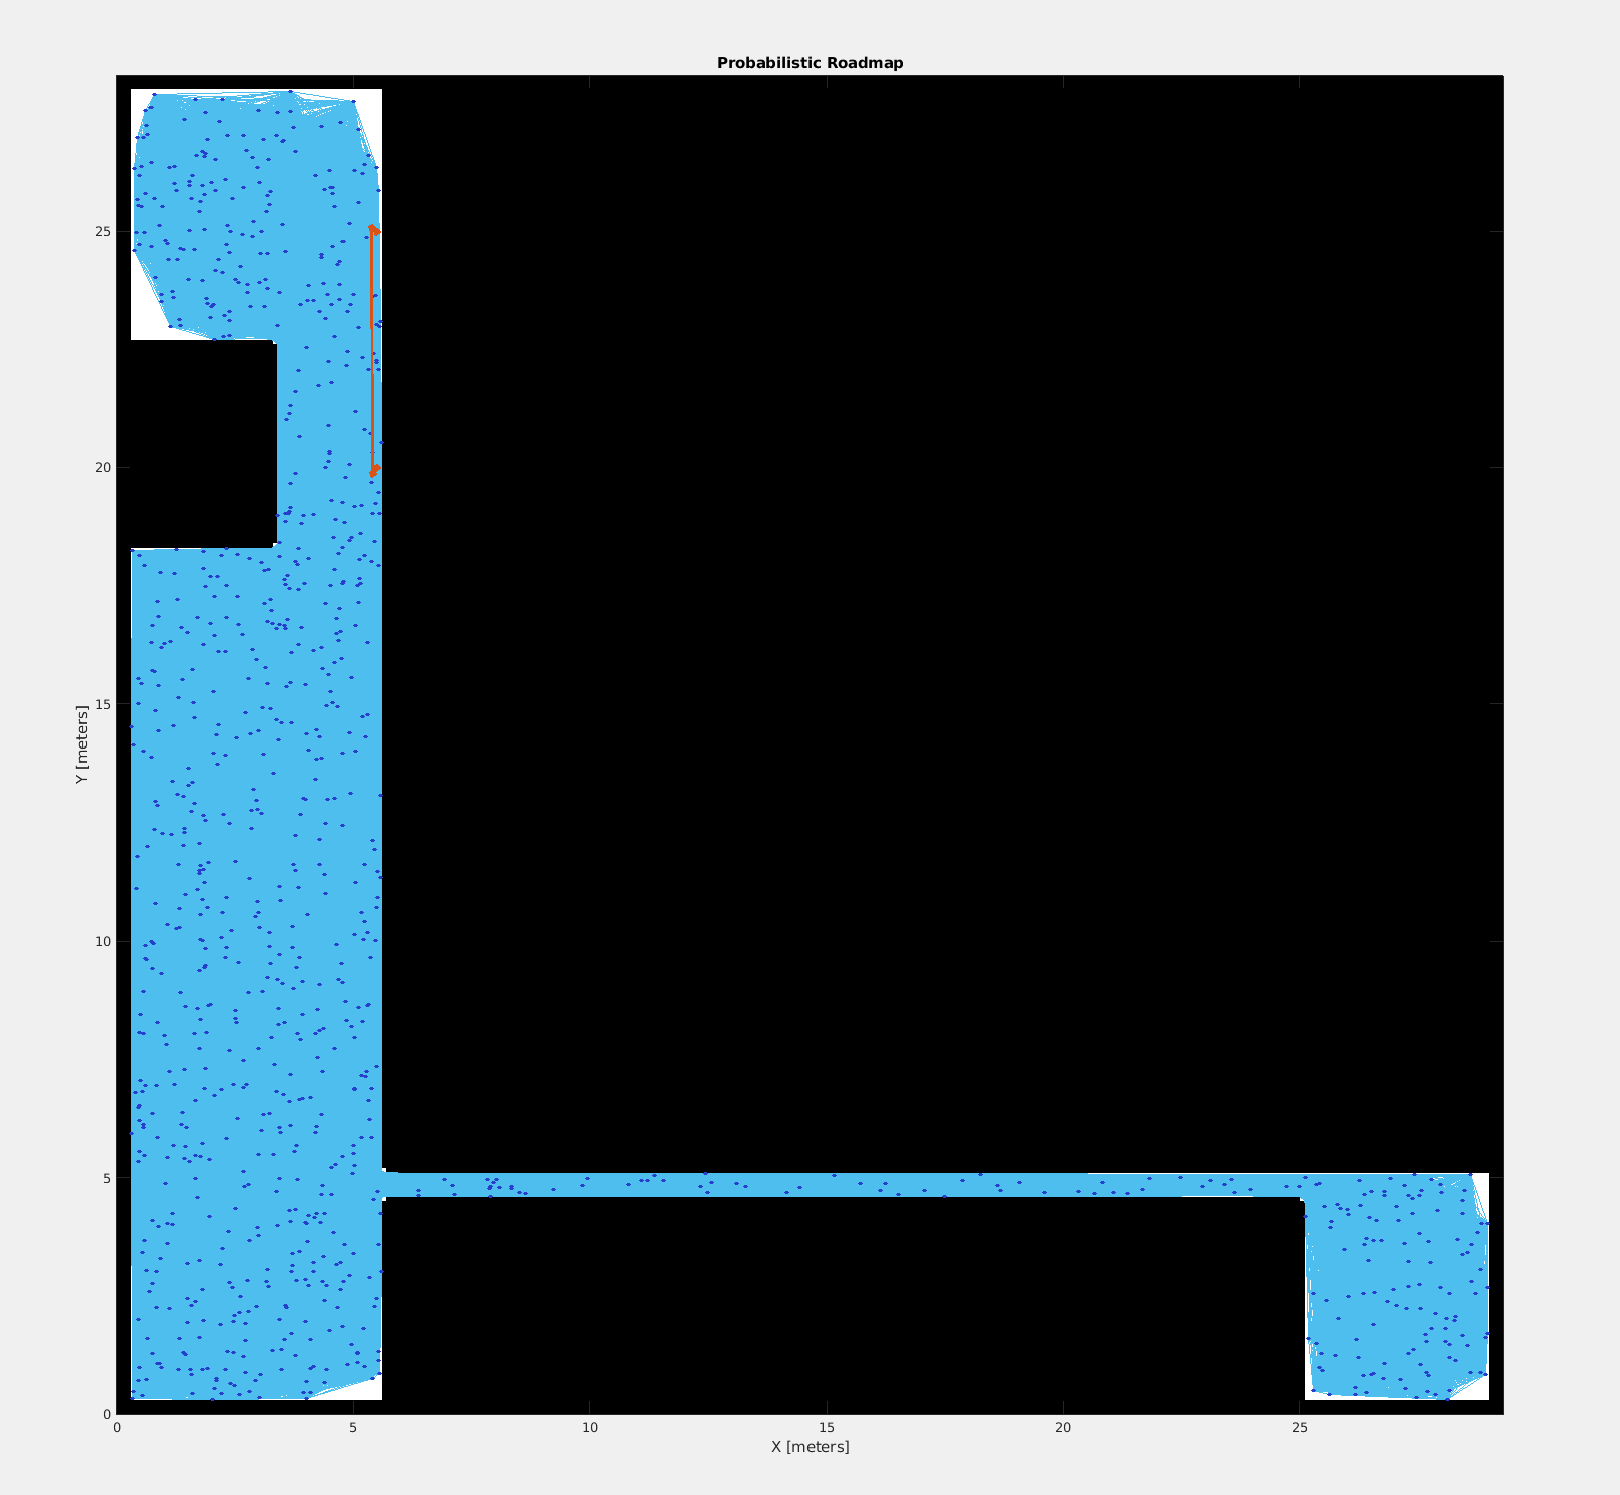
\includegraphics[width=\textwidth]{fig/fig10.png}
			\caption{PRM with mobileRobotPRM(map,1000)}
			\label{fig:fig10}
		\end{subfigure}
		\hfill
		\begin{subfigure}[b]{0.45\textwidth}
			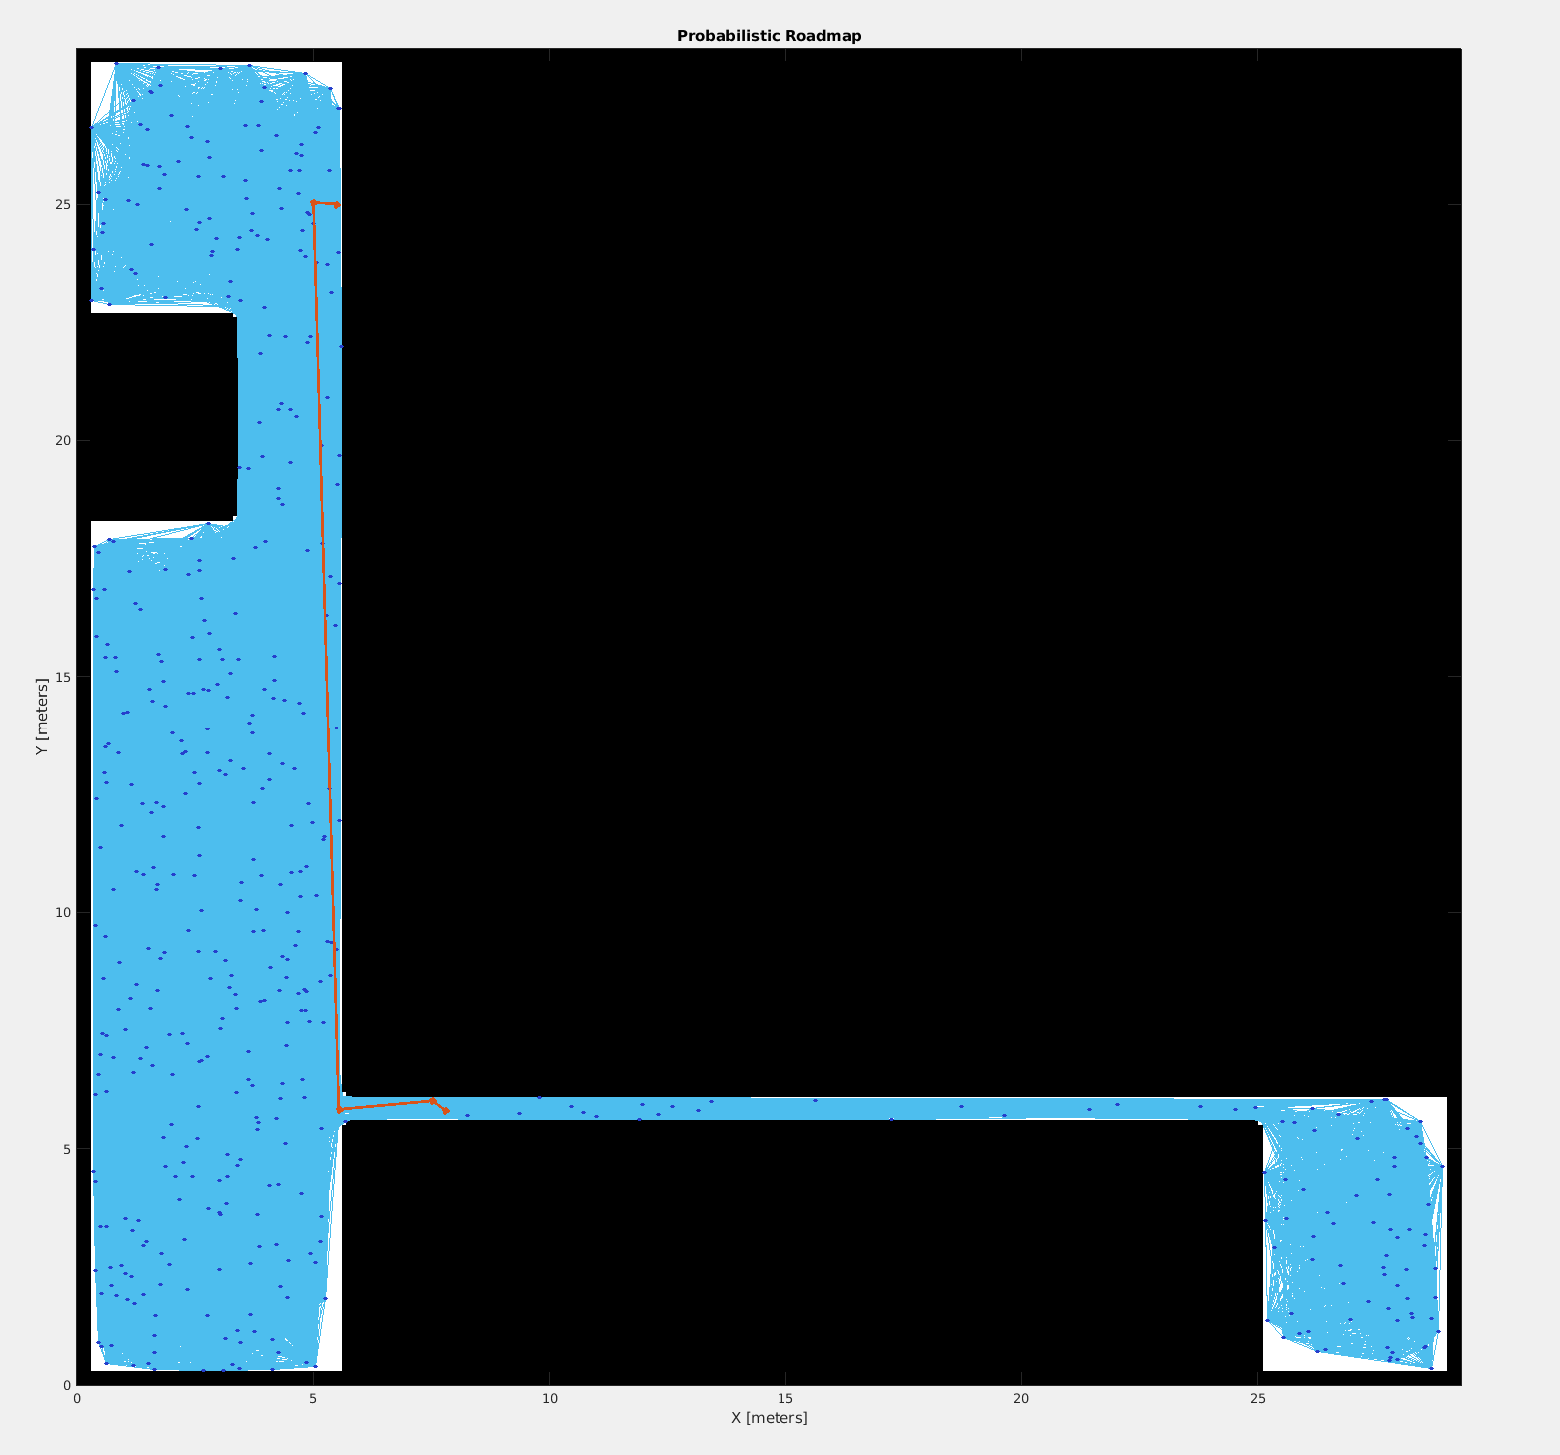
\includegraphics[width=\textwidth]{fig/fig11.png}
			\caption{PRM with mobileRobotPRM(map,500)}
			\label{fig:fig11}
		\end{subfigure}
	\end{figure}
	\subsection{Challenges and Considerations}
	\begin{itemize}
		\item \textbf{Dynamic Obstacles:} The ability to avoid dynamic obstacles requires the robot's localization system to be highly responsive and accurate in real-time.
		\item \textbf{Environmental Factors:} Changes in the environment, such as moved furniture or altered lighting conditions, can pose challenges to localization accuracy.
	\end{itemize}
	
	\subsection{Implementation of TurtleBot3's Map generating}
	The MATLAB code for generating the PRM can be found in the Appendix~\ref{appendix:code}. In these two picture we can see all the back which is static obstacles where the blue color is all the strings between possible waypoints. Each waypoint are connected to it's nearest neighbor by a straight line and are not crossing any obstacles. 
	\begin{itemize}
		\item Step 1: Defining the Binary Occupancy Map by using the function binaryOccupancyMap(29.3,28.3,10) with the following values.
		\item Step 2: For making static obstacles in the map then the following following has been used setOccupancy(map,[1,1],walls,'grid'). 
		\item Step 2: we create 500/1000 node points
		\item Step 3: finding the shortest path by using the function findpath(PRM,startLocation,endLocation)
	\end{itemize}
	
	\section{Mapping}
	Mapping is a crucial capability in robotics, particularly for autonomous navigation tasks. It involves creating a model of the robot's environment that can be used to plan and execute movements accurately. In the context of this project, the TurtleBot is required to map the Shannon building in order to navigate effectively and autonomously perform tasks in Locations B and C.
	
	\subsection{Role of Mapping in the Project}
	The mapping process for the TurtleBot involves several key functions:
	\begin{enumerate}
		\item \textbf{Environmental Model Creation:} Before the TurtleBot can begin its tasks, it needs a detailed map of the Shannon building. This map serves as the fundamental guide for all navigation and task execution.
		\item \textbf{Integration with Localization:} Mapping is closely integrated with localization; as the TurtleBot moves and captures data about its environment, it simultaneously updates its position within the map, ensuring accurate navigation.
		\item \textbf{Obstacle Identification:} The map must include information about static obstacles (like walls and furniture) and allow for the recognition and avoidance of dynamic obstacles.
	\end{enumerate}
	
	\subsection{Mapping Techniques and Technologies}
	To effectively create and utilize maps, the TurtleBot employs several advanced technologies and techniques:
	\begin{itemize}
		\item \textbf{Probabilistic Roadmap (PRM):} PRM techniques are used to construct the map and plan paths within that map. This is critical for the TurtleBot as it allows for dynamic interaction with the environment.
		\item \textbf{LiDAR and Sensors:} LiDAR sensors provide detailed and accurate distance measurements that feed into the PRM process, helping to create a precise map of the environment. Additional sensors, such as cameras, are used for detecting specific features and markers like the red and purple circles.
		\item \textbf{Path Planning Algorithms:} Once a map is created, path planning algorithms calculate the most efficient route from one point to another, considering both the mapped environment and current localization data.
	\end{itemize}
	
	\subsection{Challenges in Effective Mapping}
	Mapping in a dynamic environment like the Shannon building poses several challenges:
	\begin{itemize}
		\item \textbf{Dynamic Changes:} Changes within the building, such as moved furniture or temporary obstructions, require the TurtleBot to update its map regularly or recalibrate its path planning.
		\item \textbf{Computational Requirements:} High-resolution mapping requires significant computational resources, which can challenge the processing capabilities of onboard systems like those in the TurtleBot.
		\item \textbf{Accuracy and Resolution:} The accuracy of the map directly affects the robot's ability to perform tasks precisely, such as stopping at a specific location to take a picture.
	\end{itemize}
	
	\subsection{Applications of Mapping}
	\begin{itemize}
		\item \textbf{Task Execution:} Accurate maps are essential for precisely executing tasks, such as locating markers and navigating to specific points within the building.
		\item \textbf{Safety and Navigation:} Effective mapping ensures that the TurtleBot avoids collisions and navigates safely around people and objects.
	\end{itemize}
	In summary, mapping is a foundational aspect of this project, enabling the TurtleBot to perform its tasks with high efficiency and precision. The ability to dynamically interact with the environment through continuous mapping and localization adjustments is key to the success of the TurtleBot's operations in the Shannon building.
	
	\subsection{Implementation Of Mapping}
	The MATLAB code in Appendix~\ref{appendix:code} demonstrates how the map was created.
	
	\section{Obstacle Avoidance}
	A range of techniques were implemented to handle both static and dynamic obstacles. These techniques ensure that the robot can navigate safely and efficiently in a dynamic environment such as the Shannon building.
	
	\subsection{Static Obstacles}
	Static obstacles are elements in the environment that do not change position over time, such as walls, furniture, and other fixed structures. To handle these, the following techniques were used:
	
	\subsubsection{Probabilistic Roadmap (PRM)}
	PRM was used to generate a map of the environment and plan paths from a starting position to a destination. PRM works by creating a graph of possible paths through random sampling of the environment and connecting these points in a way that avoids known static obstacles.
	
	\subsubsection{Pure Pursuit Controller}
	The Pure Pursuit Controller is used to follow the planned path generated by the PRM. The controller continuously calculates the necessary steering angle to follow the path, ensuring that the robot stays on a safe path free of static obstacles.
	
	\subsubsection{Wall Following}
	The function \texttt{follow\_wall} uses LiDAR data to find and follow walls. The robot adjusts its course to maintain a certain distance from the wall, helping to avoid collision risks with static obstacles. This method ensures the robot navigates effectively along corridors and around fixed objects.
	
	\subsection{Dynamic Obstacles}
	Dynamic obstacles are elements in the environment that can change position over time, such as people or other robots. To handle these, real-time adjustments based on sensor data were implemented:
	
	\subsubsection{Real-time LiDAR Data}
	The LiDAR sensor continuously collects data about the environment around the robot. This data is used to identify both static and dynamic obstacles in real-time.
	
	\subsubsection{Dynamic Path Adjustment}
	The function \texttt{follow\_wall} dynamically adjusts the robot's course when obstacles are detected. The robot continuously calculates the distance to the nearest obstacle and adjusts its movement to maintain a safe distance.
	
	\subsubsection{Aiming Point Calculation}
	The robot defines an aiming point that is safe from obstacles and adjusts its course to reach this point. This mechanism ensures that the robot can navigate safely around both static and dynamic obstacles.
	
	\subsection{Implementation Details}
	Here is an overview of the implementation of obstacle avoidance in the code. For the complete code, please refer to the appendix under the specified function names.
	
	\subsubsection{PRM Generation}
	The creation of the probabilistic roadmaps is handled by the functions \texttt{createFirstPRM} and \texttt{createSecondPRM}. These functions generate maps and paths that the robot can follow while avoiding static obstacles.
	
	\subsubsection{Wall Following}
	The \texttt{follow\_wall} function is used to follow walls and avoid obstacles dynamically. It uses real-time LiDAR data to adjust the robot's path.
	
	\subsubsection{Circle Detection and Path Adjustment}
	The functions \texttt{look\_for\_circle} and \texttt{drive\_to\_circle\_and\_take\_picture} handle the detection of target objects (circles) and adjust the robot's path accordingly to avoid obstacles while approaching these targets.
	\\\\
	This combination of techniques and real-time data ensures that the robot can navigate in the given environment, handle both static and dynamic obstacles, and complete its tasks.
	

	\section{Discussion}
	On the demo day, the robot successfully demonstrated the localization and navigation process using PRM and Pure Pursuit. Initially, the robot generated a probabilistic roadmap (PRM) to model the Shannon building environment. With this roadmap, it planned a route from Location A to Location B and utilized the Pure Pursuit controller to navigate along the planned path. Upon reaching Location B, the robot successfully detected a red circle on the wall, approached it, and took a picture as required.
	\\\\
	After completing the task at Location B, the robot generated a new PRM to plan the route to Location C. During this journey, the obstacle avoidance functionality was tested, demonstrating the robot's ability to navigate around dynamic obstacles. However, an issue arose when the robot encountered a glass partition. The glass, being transparent, was not detected correctly by the sensors, necessitating manual intervention to obscure the glass and allow the robot to proceed.
	\\\\
	Upon arrival at Location C, the robot failed to detect the purple circle. This failure was likely due to insufficient tuning of the color detection thresholds, compounded by challenging lighting conditions that hindered the camera's ability to distinguish the purple color accurately.
	\\\\
	An important consideration for future improvements is the management of sensor data processing. In the current implementation, all sensor data processing runs within a single thread. This can lead to delays and reduced responsiveness, especially when handling real-time data from multiple sensors. To enhance the robot's performance, all sensor-related tasks could be run in separate threads. This multithreading approach would allow for more efficient and timely processing of sensor data, leading to better obstacle detection and avoidance, as well as more accurate localization and navigation.
	
	\section{Conclusion}
	The project successfully demonstrated autonomous navigation and object detection capabilities, despite several challenges. The primary issues encountered included difficulties with color detection thresholds and environmental factors such as lighting and glass partitions. To improve the system, future work could focus on:
	
	\begin{itemize}
		\item \textbf{Exploring Alternative Map generation like SLAM:} Implementing Simultaneous Localization and Mapping (SLAM) could provide more accurate and dynamic mapping and localization.
		\item \textbf{Enhanced Circle Detection:} Spending more time fine-tuning the circle detection algorithm and adjusting thresholds to account for varying lighting conditions.
		\item \textbf{Exploring Alternative Path Planning Methods:} Investigating other path-planning algorithms such as Bug0, Bug1, and Bug2 to enhance obstacle avoidance and navigation efficiency.
	\end{itemize}
	Despite the hardware challenges, the robot successfully completed its tasks, demonstrating robust localization and navigation capabilities. The experience highlighted the importance of adapting to environmental conditions and the potential for further improvements in autonomous robotics.
	\clearpage
	\appendix
	\section{MATLAB Code for Localization and Mapping}
	\label{appendix:code}
	\begin{verbatim}
		%% Add Path for Includes
		addpath('eksamen_includes.m');
		
		%% Set Environment Variables for ROS
		setenv('ROS_MASTER_URI','http://192.168.252.100:11311');
		setenv('ROS_IP','192.168.252.38');
		
		%% Initialize ROS
		rosshutdown()  % Shutdown any previous ROS instance
		rosinit('http://192.168.252.100:11311','NodeHost','192.168.252.38')
		
		%% Subscriber and Publisher Setup
		% Subscribe to the camera topic
		cam_sub = rossubscriber('/usb_cam/image_raw/compressed',"DataFormat", "Struct");
		
		% Publisher for velocity commands
		vel_pub = rospublisher('/cmd_vel');
		
		% Subscribe to the LiDAR scan topic
		scansub = rossubscriber('/scan');
		
		% Subscribe to the transform topic for position updates
		pos_sub = rossubscriber('/tf');
		
		% Publisher to reset the robot
		reset_pub = rospublisher('/reset');
		send(reset_pub, rosmessage(reset_pub));
		
		%% Controller Setup
		controller = controllerPurePursuit;
		controller.DesiredLinearVelocity = 0.2;
		controller.MaxAngularVelocity = 2;
		
		% We found that the robot is relatively stable with a LookAheadDistance of 0.4
		controller.LookaheadDistance = 0.4;
		
		% Since we're using the reference frame of the LiDAR, position and angle are always 0
		
		%% Create PRMs for Path Planning
		first_PRM = createFirstPRM();
		second_PRM = createSecondPRM();
		
		%% Initialize State and Parameters
		ZONE_B_X_VALUE = 5;
		state = 1;
		drive_distance = 0.5;
		
		%% Main Control Loop
		while (1)
		switch(state)
		case 1
		follow_road_map(pos_sub, vel_pub, first_PRM);
		state = 2;
		
		case 2
		follow_wall(drive_distance, scansub, vel_pub, pos_sub, controller);
		[circle_seen, center] = look_for_circle(pos_sub, vel_pub, cam_sub);
		if (circle_seen == 1)
		drive_distance = 0.2;
		elseif (circle_seen == 2)
		state = 3;
		drive_distance = 0.5;
		else
		drive_distance = 0.5;
		end
		
		case 3
		drive_to_circle_and_take_picture(cam_sub, vel_pub, scansub);
		state = 4;
		
		case 4
		follow_road_map(pos_sub, vel_pub, second_PRM);
		state = 5;
		
		case 5
		follow_wall(drive_distance, scansub, vel_pub, pos_sub, controller);
		circle_seen = look_for_circle(pos_sub, vel_pub, cam_sub);
		state = 6;
		
		case 6
		drive_to_circle_and_take_picture(cam_sub, vel_pub, scansub);
		end
		end
		
		%% Function Definitions
		
		% Follow Wall Function
		function [true] = follow_wall(drive_distance, scansub, vel_pub, pos_sub, controller)
		start_pos = update_pos(pos_sub);
		robotCurrentPose = update_pos(pos_sub);
		
		while(norm(robotCurrentPose(1:2) - start_pos(1:2)) < drive_distance )
		
		%% Data Retrieval
		scan = receive(scansub);
		cart = readCartesian(scan);
		
		hold on
		xlim([-3 3])
		ylim([-3 3])
		
		x = cart(:, 1);  % x-pos
		d = cart(:, 2);  % y-pos
		
		% Filter out points with y coordinates above 0 (to the right of the robot)
		filtered_indices = d >= 0;
		x = x(filtered_indices);
		d = d(filtered_indices);
		
		%% Fitting the Line of the Wall and Plotting It
		mdl = fitlm(x, d);
		coef = mdl.Coefficients.Estimate;
		plot(x, (coef(1) + coef(2) * x), 'r')
		
		% Calculate the distance from the robot to the line to check if distance is ~0.5 meter
		distance = abs(coef(1)) / sqrt(1 + coef(2)^2);
		
		% Defining a point to aim for 0.5 meters out from the wall and 1 meter ahead
		aim_point = [1 (coef(2) * 1 + coef(1)) - 1];
		plot(aim_point(1), aim_point(2), 'bx');
		
		% Setting the controller to go towards the aim-point
		controller.Waypoints = aim_point;
		[v, w] = controller([0 0 0]);
		update_vel(v, w, vel_pub)
		
		robotCurrentPose = update_pos(pos_sub);
		end
		end
		
		% Look for Circle Function
		function [seen, center] = look_for_circle(pos_sub, vel_pub, cam_sub)
		start_pos = update_pos(pos_sub);
		now_pos = start_pos;
		while(abs((now_pos(3) - start_pos(3))) < 1.5)
		update_vel(0, 1, vel_pub);
		now_pos = update_pos(pos_sub);
		end
		
		update_vel(0, 0, vel_pub);
		[seen, center] = detectRedCircle(cam_sub);
		
		if seen ~= 2
		while((now_pos(3) - start_pos(3)) > 0.5)
		update_vel(0, -1, vel_pub);
		now_pos = update_pos(pos_sub);
		end
		end
		end
		
		% Create First PRM Function
		function [path] = createFirstPRM()
		map = binaryOccupancyMap(29.3, 28.3, 10);
		walls = zeros(40, 60);
		
		% Left wall
		walls(1:283, 1) = 1;
		% Right wall
		walls(1:283, 293) = 1;
		% Top wall
		walls(1, 1:293) = 1;
		% Bottom wall
		walls(283, 1:293) = 1;
		
		% Zone a and rooms next to it
		walls(1:230, 59:293) = 1;
		% Door before zone b
		walls(59:98, 1:32) = 1;
		% Rooms next to zone c and corridor
		walls(240:283, 59:249) = 1;
		
		setOccupancy(map, [1, 1], walls, 'grid')
		inflate(map, 0.2);
		PRM = mobileRobotPRM(map, 500);
		startLocation = [5.5 25];
		endLocation = [5.5 21];
		path = findpath(PRM, startLocation, endLocation);
		figure
		show(PRM)
		end
		
		% Create Second PRM Function
		function [path] = createSecondPRM()
		map = binaryOccupancyMap(29.3, 28.3, 10);
		walls = zeros(40, 60);
		
		% Left wall
		walls(1:283, 1) = 1;
		% Right wall
		walls(1:283, 293) = 1;
		% Top wall
		walls(1, 1:293) = 1;
		% Bottom wall
		walls(283, 1:293) = 1;
		
		% Zone a and rooms next to it
		walls(1:230, 59:293) = 1;
		% Door before zone b
		walls(59:98, 1:32) = 1;
		% Rooms next to zone c and corridor
		walls(240:283, 59:249) = 1;
		
		setOccupancy(map, [1, 1], walls, 'grid')
		inflate(map, 0.2);
		PRM = mobileRobotPRM(map, 500);
		startLocation = [5.5 25];
		endLocation = [25.5 3.5];
		path = findpath(PRM, startLocation, endLocation);
		figure
		show(PRM)
		end
		
		% Follow Road Map Function
		function [true] = follow_road_map(pos_sub, vel_pub, path)
		%% Controller Setup
		controller = controllerPurePursuit;
		controller.DesiredLinearVelocity = 0.2;
		controller.MaxAngularVelocity = 2;
		
		% We found that the robot is relatively stable with a LookAheadDistance of 0.4
		controller.LookaheadDistance = 0.4;
		goalRadius = 0.5;
		robotCurrentPose = update_pos(pos_sub);
		distanceToGoal = norm(robotCurrentPose - path(end, :))
		
		controller.Waypoints = path;
		
		while(distanceToGoal > goalRadius)   
		
		% We start the loop by updating the position of the robot
		Pose = update_pos(pos_sub);
		
		robotCurrentPose = [Pose(1) + 5.5; Pose(2) + 25; Pose(3)];
		
		% Compute the controller outputs, i.e., the inputs to the robot
		[v, w] = controller(robotCurrentPose);
		
		% Then we update the angular and linear velocities based on the controller outputs.
		update_vel(v, w, vel_pub)
		
		% At last we check the distance to goal for whether we have reached the end of the path.
		distanceToGoal = norm(robotCurrentPose(1:2) - path(end, :)')
		end
		end
		
		% Drive to Circle and Take Picture Function
		function [true] = drive_to_circle_and_take_picture(cam_sub, vel_pub, scansub)
		[found, center] = detectRedCircle(cam_sub);
		distanceToWall = 1;
		
		while(center > 320)
		[found, center] = detectRedCircle(cam_sub);
		update_vel(0, 0.1, vel_pub);
		end
		
		while(center < 320)
		[found, center] = detectRedCircle(cam_sub);
		update_vel(0, 0.1, vel_pub);
		update_vel(0, -0.1, vel_pub);
		end
		
		while(distanceToWall > 0.5)
		[found, center] = detectRedCircle(cam_sub);
		
		if(center > 320)
		update_vel(0.1, 0.05, vel_pub);
		else
		update_vel(0.1, -0.05, vel_pub);
		end
		
		%% Data Retrieval
		scan = receive(scansub);
		cart = readCartesian(scan);
		
		hold on
		xlim([-3 3])
		ylim([-3 3])
		
		x = cart(:, 1);  % x-pos
		d = cart(:, 2);  % y-pos
		
		% Filter out points with x coordinates above 0 (to the front of the robot)
		filtered_indices = x >= 0;
		x = x(filtered_indices);
		d = d(filtered_indices);
		
		%% Fitting the Line of the Wall and Plotting It
		mdl = fitlm(x, d);
		coef = mdl.Coefficients.Estimate;
		
		% Calculate the distance from the robot to the line to check if distance is ~0.5 meter
		distanceToWall = abs(coef(1)) / sqrt(1 + coef(2)^2);
		disp(distanceToWall)
		end
		end
		
		% Update Velocity Function
		function [true] = update_vel(v, w, vel_pub)
		% Very simple function. We get a new linear and angular velocity from the controller and output it to the cmd_vel topic.
		twistmsg = rosmessage(vel_pub);
		
		twistmsg.Angular.Z = w;
		twistmsg.Linear.X = v;
		
		send(vel_pub, twistmsg);
		end
		
		% Update Position Function
		function [output] = update_pos(pos_sub)
		% We start by getting the transform data from the tf topic
		receive(pos_sub, 10);
		
		% the x and y data is = to the x and y of the tf topic
		pos.x = pos_sub.LatestMessage.Transforms.Transform.Translation.X;
		pos.y = pos_sub.LatestMessage.Transforms.Transform.Translation.Y;
		
		% We use the function quat2angle to transform the angle from quaternion to yaw in radians
		quat.X = pos_sub.LatestMessage.Transforms.Transform.Rotation.X;
		quat.Y = pos_sub.LatestMessage.Transforms.Transform.Rotation.Y;
		quat.Z = pos_sub.LatestMessage.Transforms.Transform.Rotation.Z;
		quat.W = pos_sub.LatestMessage.Transforms.Transform.Rotation.W;
		
		[roll, pitch, yaw] = quat2angle([quat.X, quat.Y, quat.Z, quat.W]);
		
		pos.theta = yaw;
		
		% In the end we output the data and add the initial position of the robot to x and y
		output = [pos.x; pos.y; pos.theta];
		end
		
		% Detect Colored Circle Function
		function [circleFound, circleColor, confidence] = detectColoredCircle(img)
		% Convert the image to grayscale
		grayImg = rgb2gray(img);
		
		% Use morphological erosion and then dilation to enhance image processing, optional
		se = offsetstrel('ball', 5, 5);
		imgProcessed = imdilate(imerode(grayImg, se), se);
		
		% Find circles in the image
		[centers, radii, metric] = imfindcircles(imgProcessed, [10 100], 'ObjectPolarity', 'dark', 'Sensitivity', 0.85);
		
		% Initialize output variables
		circleFound = false;
		circleColor = '';
		confidence = 0;
		
		% Check if any circles were found
		if ~isempty(centers)
		circleFound = true;
		confidence = max(metric);  % Maximum confidence value from detections
		
		% Assume the circle with the highest confidence is the one we are interested in
		bestCircleIndex = find(metric == max(metric), 1);
		bestCircleColor = impixel(img, centers(bestCircleIndex, 1), centers(bestCircleIndex, 2));
		
		% Define thresholds for red and purple color
		redThresholdLow = [150, 0, 0];
		redThresholdHigh = [255, 100, 100];
		purpleThresholdLow = [75, 0, 75];
		purpleThresholdHigh = [140, 80, 150];
		
		% Check the color within the best circle
		if all(bestCircleColor(1, :) >= redThresholdLow) & all(bestCircleColor(1, :) <= redThresholdHigh)
		circleColor = 'Red';
		elseif all(bestCircleColor(1, :) >= purpleThresholdLow) & all(bestCircleColor(1, :) <= purpleThresholdHigh)
		circleColor = 'Purple';
		else
		circleColor = 'Other';
		end
		end
		
		% Visualize the detection
		imshow(img);
		hold on;
		viscircles(centers, radii, 'EdgeColor', 'b');
		hold off;
		title(sprintf('Detected Circle: %s (%.2f%% Confidence)', circleColor, confidence * 100));
		end
		
		% Detect Red Circle Function
		function [found, center] = detectRedCircle(cam_sub)
		imgraw = receive(cam_sub); % a serialized compressed image
		
		input_image = imrotate(rosReadImage(imgraw), 180, "bilinear");
		
		imwrite(input_image, 'test_image.jpg');
		
		% input_image = imread("test_image.jpg");
		
		% Convert the image from RGB to HSV color space
		hsv_image = rgb2hsv(input_image);
		
		% Define thresholds for the hue, saturation, and value channels
		hue_threshold = [0 0.1]; % Values for red hues
		saturation_threshold = [0.5 1]; % Minimum saturation to avoid grays/blacks
		value_threshold = [0.5 1]; % Full range of value
		
		% Create a mask using the threshold values
		hue_mask = (hsv_image(:,:,1) >= hue_threshold(1)) & (hsv_image(:,:,1) <= hue_threshold(2));
		saturation_mask = (hsv_image(:,:,2) >= saturation_threshold(1)) & (hsv_image(:,:,2) <= saturation_threshold(2));
		value_mask = (hsv_image(:,:,3) >= value_threshold(1)) & (hsv_image(:,:,3) <= value_threshold(2));
		
		% Combine the masks
		final_mask = hue_mask & saturation_mask & value_mask;
		
		% Apply the mask to the original image
		output_image = input_image;
		output_image(repmat(~final_mask, [1 1 3])) = 0; % Set non-masked pixels to black
		
		SE = strel('disk', 5);
		
		output_image = imerode(output_image, SE);
		output_image = imdilate(output_image, SE);
		
		gray_image = rgb2gray(output_image);
		
		output_image = gray_image > 0;
		
		[centers, radii, confidence] = imfindcircles(output_image, [10 200]);
		
		% Display the original and thresholded images
		subplot(1, 2, 1);
		imshow(input_image);
		title('Original Image');
		
		if ~isempty(confidence)
			center = centers(1);
			if(confidence(1) > 0.1)
			viscircles(centers(1, :), radii(1), 'EdgeColor', 'b'); 
			found = 1;
		end
		
		if(confidence(1) > 0.3)
			found = 2;
			end
			else
			found = 0;
			center = [0 0];
		end
		
		% Visualize the detection
		hold on;
		subplot(1, 2, 2);
		imshow(output_image);
		title('Thresholded Image');
		end
	\end{verbatim}
	\subsection{Task provided by the school}
	\label{appendix:task}
	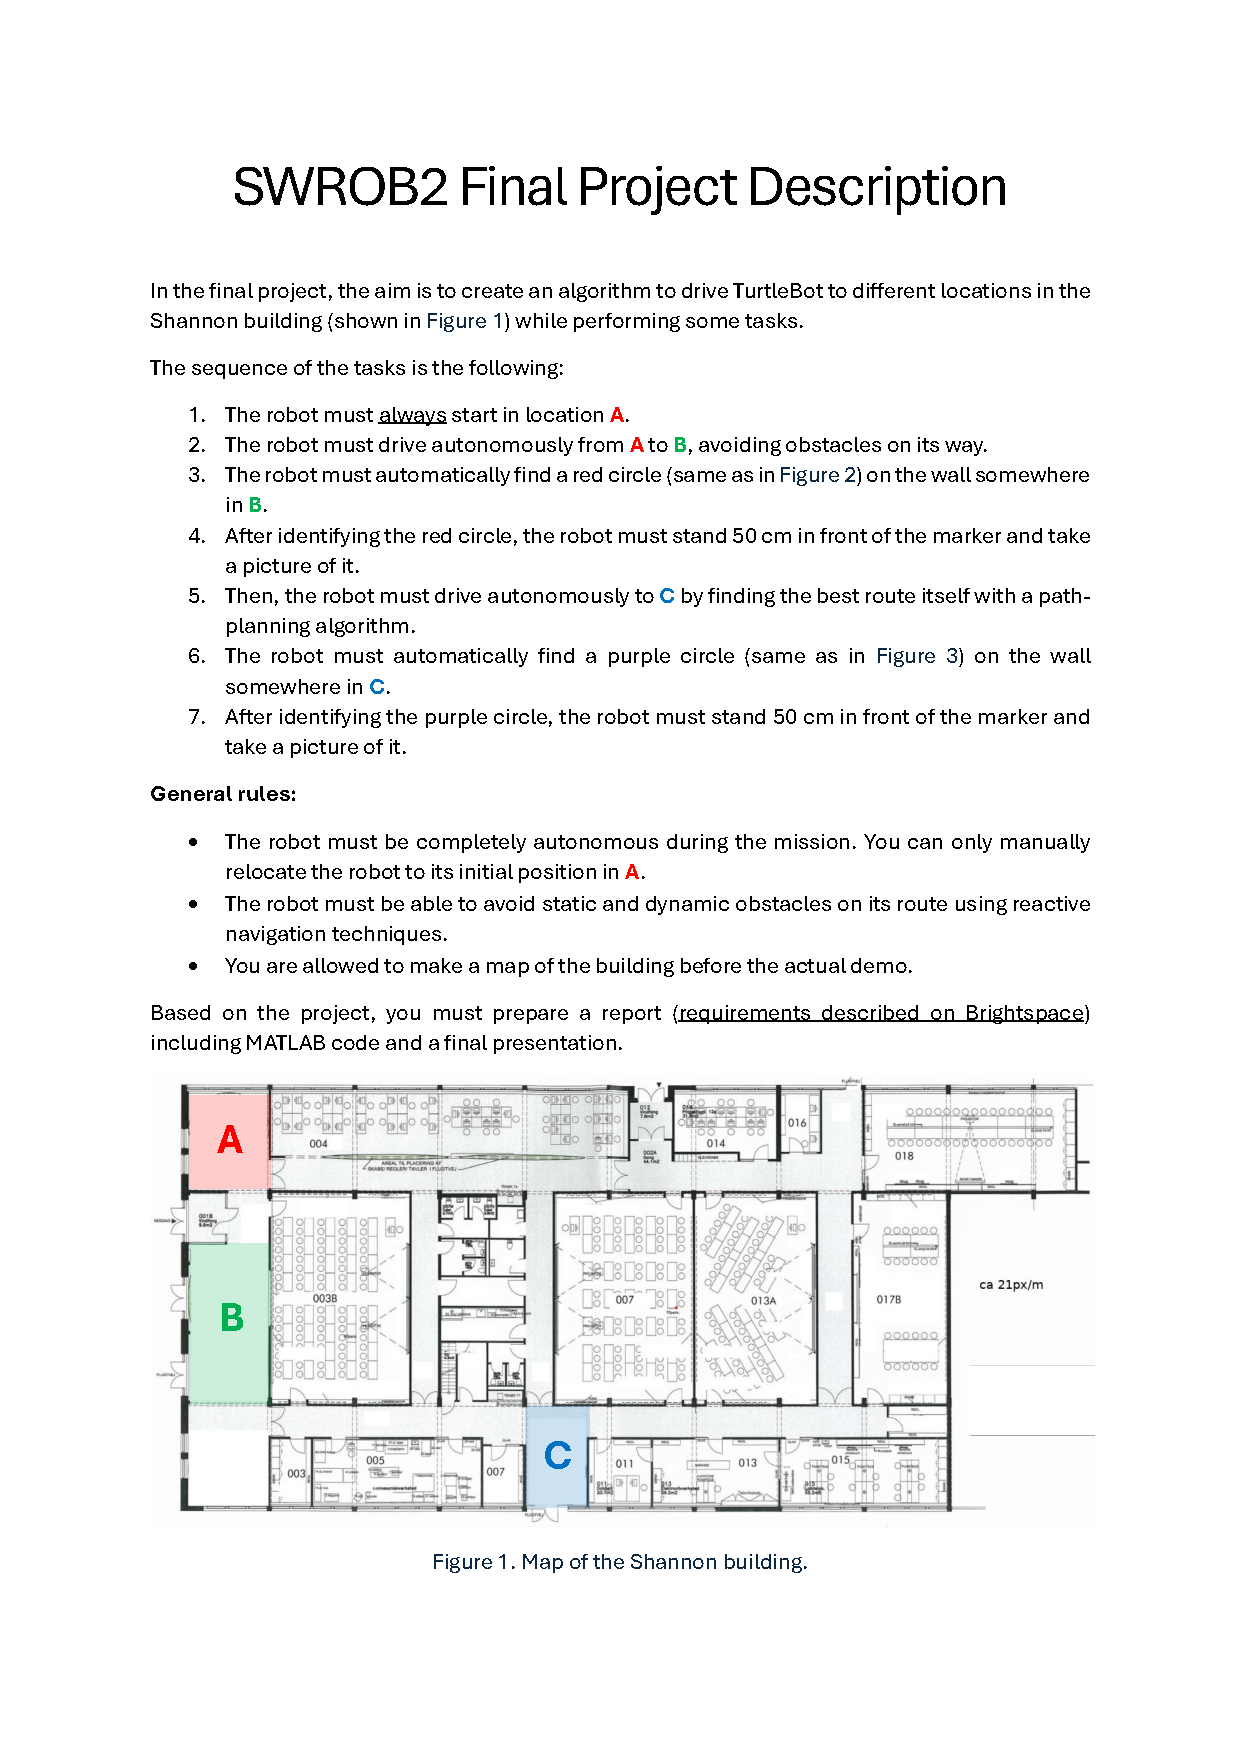
\includepdf{SWROB2 Final Project Description 2024.pdf}
\end{document}
